\chapter{Omräkning mellan dB och kvoten av tal}
\label{decibel}

Benämningen Bel kommer från namnet på amerikanen Alexander Graham
Bell, som år 1876 uppfann den första praktiskt användbara telefonen
efter ideer från tysken Philipp Reiß.

Inom teletekniken används begreppet decibel för att beskriva förlopp
av effekt, ström och spänning.  Begreppet förekommer även i andra
sammanhang, t.ex. akustik där det istället är fråga om ljudtryck.

Måtten i det metriska systemet är alldagliga och ingen finner det
märkligt att det t.ex. går tio decimeter på en meter. Däremot är
begreppet decibel ovant för många.

Räkning med decibel grundas på användning av logaritmer, som är ett
bekvämt sätt att uttrycka och behandla talvärden.  Detta har i
korthet förklarats i avsnitt \ref{effect och energi}.  Här beskrivs ett
omräkningsförfarande med hjälp av tabeller.

\emph{Decibel är ett dimensionslöst uttryck för graden av dämpning
  alternativt förstärkning.}

\emph{Dämpning är följden av att vissa komponenter bromsar elektrisk
  ström.}

\emph{Förstärkning innebär att en aktiv komponent kan styra en större
  elektrisk ström och därmed större effekt än den själv styrs med.}

\section{Bestämning av dB ur effektförhållandet}

\begin{rev-raderas}

$>>>>>$ TODO: Förfarandet som beskrivs här för omvandling dB-spänning är otroligt krångligt, föreslår att vi istället har en kort tabell (eller nomogram), samt hänvisar till hur man slår på en miniräknare


\begin{enumerate}
\item Dela upp effektförhållandet i faktor och 10-potens
\item Bestäm dB-talet för 10-potensen
\item Bestäm dB-talet för faktorn med nomogram (se bild
  \ref{nomogram-db-spänning}), tabell eller räknare
\item Addera dB-talen till ett slutresultat
\end{enumerate}

Exempel: dB-talet för 300-faldig effekt\emph{förstärkning}
\begin{enumerate}
\item \(300 = 3 \cdot 100\)
\item 100 motsvarar 20 dB
\item 3 motsvarar 4.8 dB
\item \(20 + 4.8 = +24.8\) dB
\end{enumerate}

Exempel: dB-talet för 70 000-faldig effektminskning
\begin{enumerate}
\item 70 000 = 7 . i 000
\item 10 000 motsvarar 40 dB
\item 7 motsvarar 8.5 dB
\item 40 + 8.5 =- 48.5 dB
\end{enumerate}

Exempel: En Vagi-antenn omfördelar den utstrålade effekten så att den
i bästa riktningen blir 56-faldigt bättre än från en
referensantenn. Hur många dB motsvarar det?

\[ 56 = 5.6 \cdot 10\]

vilket motsvarar

\[ 7.5 dB + 10 dB = 17.5 dB\]

Exempel: I en koaxialkabel förloras hälften av den inmatade
effekten. Hur stor är dämpningen i dB?

Effektförhållandet är faktor 2 (inverterat), d.v.s 3~dB dämpning =
-3~dB.

\end{rev-raderas}

\section{Bestämning av effektförhållandet ur dB}

\begin{rev-raderas}

\begin{enumerate}
\item Dela upp dB-talet i 1-tal och 10-tal
\item 1-talet dB ger en faktor
\item 10-talet dB ger antal nollor bakom faktorn (ställvärdet)
\item Multiplicera faktorn med ställvärdet (antalet nollor).
\end{enumerate}

Exempel: Vilket effektförhållande motsvarar 13 dB?

\begin{enumerate}
\item 13 dB = 10 dB + 3 dB
\item 3 dB motsvarar faktor 2
\item 10 dB ger 1 nolla
\item \(2 \cdot 10 = 20\), d v s 20-faldig förstärkning
\end{enumerate}

Exempel: Vilket effektförhållande motsvarar -115d8?
\begin{enumerate}
\item 15 dB = 110 + 5 dB
\item 5 dB motsvarar faktor 3.2
\item 110 dB ger 11 nollor
\item Efter decimaltecknet i faktor 3.2 följer ett ställvärde av 11 ,
  d.v.s. 320 000 000 000-faldig dämpning.
\end{enumerate}

Exempel: Om ineffekten till ett slutsteg är 100~W och det har en
förstärkning av 10~dB.  Hur stor är uteffekten?

10 dB motsvarar en 10-faldig förstärkning.  Uteffekten från slutsteget
blir således \(10 \cdot 100 = 1000\) W.

Sambandet mellan effektförhållande och dB

\begin{tabular}{l|llllllll}
  dB & 0 & & 10 & 20 & 30 & 40 & 50 & 60 \\
  \hline
  0  & 1 & & 0  & 0  & 0  & 0  & 2  & 0 \\
  1  & 1 & & 2  & 5  & 8  & 9  & 9  & 5 \\
  2  & 1 & & 5  & 8  & 4  & 8  & 6  & 3 \\
  3  & 1 & & 9  & 9  & 5  & 2  & 8  & 2 \\
  4  & 2 & & 1  & 1  & 1  & 8  & 7  & 6 \\
  5  & 3 & & 6  & 6  & 2  & 2  & 7  & 8 \\
  6  & 3 & & 8  & 8  & 1  & 0  & 7  & 2 \\
  7  & 5 &.& 1  & 1  & 1  & 8  & 7  & 2 \\
  8  & 6 & & 0  & 0  & 9  & 5  & 7  & 3 \\
  9  & 7 & & 4  & 1  & 3  & 2  & 8  & 2 \\
\end{tabular}

Kolumnen längst till vänster upptar 1-tal dB från 0 till 9 och den
översta raden upptar 10-tal dB-tal från 0 till 60.

Med tabellen kan effektförhållanden bestämmas ur dB-tal från 0 till 69
eller omvänt.  Det motsvarar effektförhållanden från 1:1 till 1:8
millioner.

Var uppmärksam på decimaltecknets placering. Avkorta till önskat antal decimaler.

Exempel: Vilket effektförhållande motsvarar +7dB?

7 ligger mellan 0 och 9. Sök därför 0 dB i den översta raden. Gå sedan
rakt nedåt i kolumnen till raden för 7 dB. Vi kommer då till första
siffran i kvoten för 7 dB. Decimaltecknet står till höger om denna
ruta (mellan kolumnerna för 0 och 10 dB).

I sifferfältet kan nu utläsas en effektförstärkning (kvot) av
5.011872.

\end{rev-raderas}

\begin{rev-raderas}

\section{Bestämning av dB ur ström- eller spänningsförhållandet}

\begin{itemize}
\item Dela upp ström- eller spänningsförhållandet i faktor och 10-potens
\item Bestäm dB-talet för 10-potensen
\item Bestäm dB-talet förfaktorn ur nomogrammet (se bild \ref{nomogram-db-spänning})
\item Addera dB-talen till ett slutresultat
\end{itemize}

Exempel: 300-faldig spänningsförstärkning
\begin{itemize}
\item \(300 = 3 \cdot 100\)
\item 100 motsvarar 40 dB, d.v.s två (nollor) gånger 20 = 40
\item 3 motsvarar 9.5 dB
\item 40 dB + 9.5 dB = 49.5 dB
\end{itemize}

\section{Bestämning av ström- eller spänningsförhållandet ur dB}
\begin{itemize}
\item Dela dB-värdet med 20 dB varvid erhålls en del och en rest
\item Delen ger 10-potensen, d.v.s antalet nollor bakom faktorn
  (ställvärdet)
\item Gå in i nomogrammet och omvandla ``resten'' till en faktor
\item Multiplicera faktorn med ställvärdet
\end{itemize}

Exempel: Vilket spänningsförhållande motsvarar -115 dB?
\begin{itemize}
\item 115 dB/20 dB= 5 rest 15
\item 5 (nollor) motsvarar 100 000
\item 5 dB motsvarar 5.5
\item \(5.5 \cdot 1 00 000\) = 550 000-faldig spänningsdämpning
\end{itemize}

\end{rev-raderas}

\begin{rev-raderas}
\section{Tabeller för sambandet mellan ström- eller spänningsförhållande
  och dB}

Kolumnerna längst till vänster upptar dB-talen 0-9. I tabellernas
översta rad är dB-talen listade i jämna 10-tal dB från O-120
respektive i udda 10-tal dB från 10-130.

Med tabellerna kan ström- och spänningsförhållanden bestämmas ur
dB-tal från 0 till 139 dB och omvänt.

Detta motsvarar förhållanden från 1:1 till 1:8.9 millioner.

Se tabell \ref{tab:db-jämna-0-120}.

\end{rev-raderas}
\begin{rev-raderas}

\begin{table}[h]
  \caption{Jämna 10-tal dB från 0 till 120 dB}
  \label{tab:db-jämna-0-120}
  \begin{tabular}{l|lllllll}
    dB & 0 & 20 & 40 & 60 & 80 & 100 & 120 \\
    \hline
    0 & 0 & 0 & 0 & 0 & 0 & 0 & 0 \\
    1 & 1 & 1 & 2 & 2 & 0 & 1 & 8 \\
    2 & 1 & 2 & 5 & 8 & 9 & 2 & 5 \\
    3 & 1 & 4 & 1 & 2 & 5 & 3 & 8 \\
    4 & 1 & 5 & 8 & 4 & 8 & 9 & 3 \\
    5 & 1 & 7 & 7 & 8 & 2 & 7 & 9 \\
    6 & 1 & 9 & 9 & 5 & 2 & 6 & 2 \\
    7 & 2 & 2 & 3 & 8 & 7 & 2 & 1 \\
    8 & 2 & 5 & 1 & 1 & 8 & 8 & 6 \\
    9 & 2 & 8 & 1 & 8 & 3 & 8 & 3 \\
  \end{tabular}
\end{table}



\begin{table}[h]
  \caption{Udda 10-tal dB från 10 till 130 dB}
  \label{tab:db-udda-10-130}
  \begin{tabular}{l|lllllll}
    dB & 10 & 30 & 50 & 70 & 90 & 110 & 130 \\
    \hline
    0 & 3 & 1 & 6 & 2 & 2 & 7 & 8 \\
    1 & 3 & 5 & 4 & 8 & 1 & 3 & 4 \\
    2 & 2 & 9 & 8 & 1 & 0 & 7 & 2 \\
    3 & 4 & 4 & 6 & 6 & 8 & 3 & 6 \\
    4 & 5 & 0 & 1 & 1 & 8 & 7 & 2 \\
    5 & 5 & 6 & 2 & 3 & 4 & 1 & 2 \\
    6 & 6 & 3 & 0 & 9 & 5 & 7 & 3 \\
    7 & 7 & 0 & 7 & 9 & 4 & 6 & 8 \\
    8 & 7 & 9 & 4 & 3 & 2 & 8 & 2 \\
    9 & 8 & 9 & 1 & 2 & 5 & 0 & 9 \\
  \end{tabular}
\end{table}

\end{rev-raderas}
\begin{rev-raderas}

Exempel:

En förstärkare med lika in- och utgångsimpedans förstärker spänningen
350-falt.  Hur många dB är det?

Vi söker närmaste 3-ställiga tal i de två ovanstående tabellerna. I
den nedersta tabellen finner vi talet 354 på andra raden.  Över
entalet 4 finner vi 50 dB i den översta raden. Till vänster om 354
finner vi 1 dB.  Som ett närmevärde är alltså förstärkningen 50 + 1 =
51~dB.

Om kvoten i nomogram i bild \ref{nomogram-db-soänning} är en eller flera 10-potenser högre
än 10 (ggr), så kan nomogrammet utökas enligt följande tabell.

\begin{tabular}{llll}
  Kvot * & Analys              & Skriv           & dB \\
  1      & 1 har 0 nollor      & \(0 \cdot 20\) = & 0  \\
  10     & 10 har 1 nolla      & \(1 \cdot 20\) = & 20 \\
  100    & 100 har 2 nollor    & \(2 \cdot 20\) = & 40 \\
  1 000  & 1 000 har 3 nollor  & \(3 \cdot 20\) = & 60 \\
  10 000 & 10 000 har 4 nollor & \(4 \cdot 20\) = & 80 \\
\end{tabular}

* kvot av \(U_{hög}/U_{låg}\) resp. \(I_{hög}/I_{låg}\).

\begin{figure}
  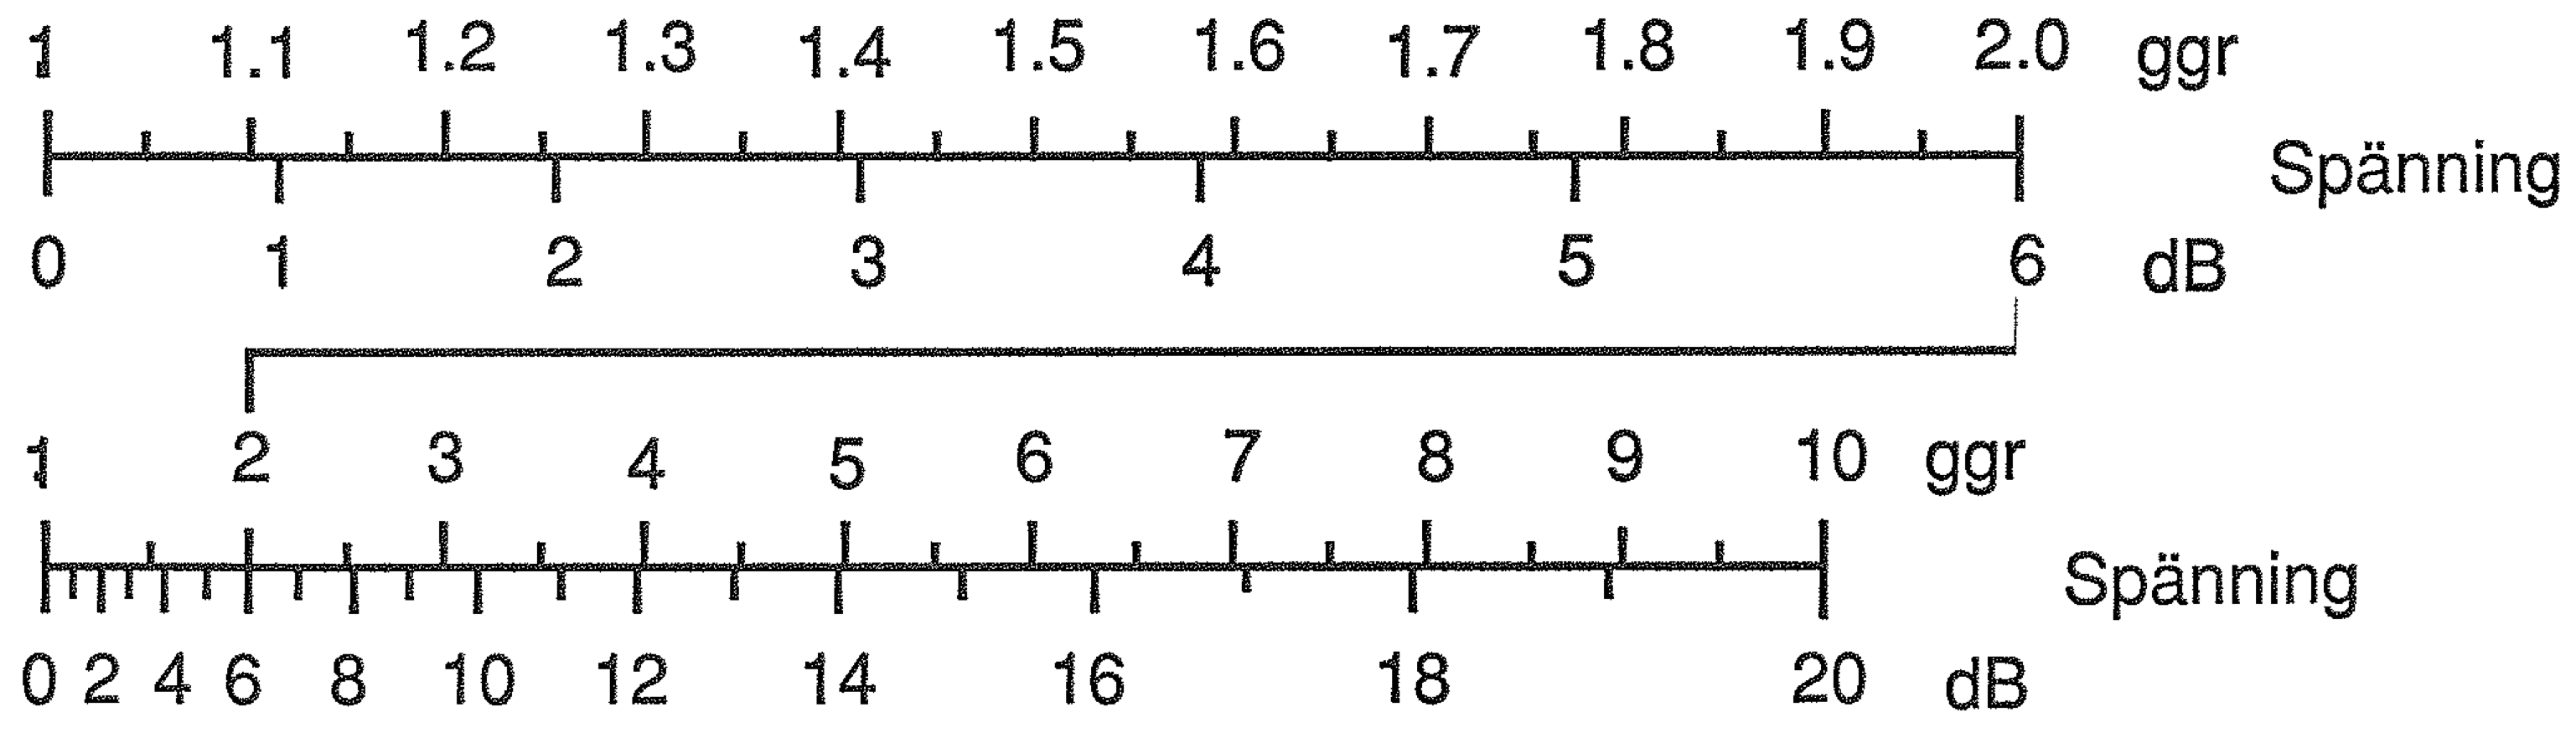
\includegraphics[width=\textwidth]{images/bild_appendix_c_nomogram}
  \caption{Nomogram för omvandling mellan spänning och decibel}
  \label{nomogram-db-spänning}
\end{figure}

\end{rev-raderas}

\section{Decibel över 1 m W vid 50 Ω [dB(m)]}

Som nu beskrivits är uttrycket decibel ett logaritmiskt mått för hur
två effekter förhåller sig till varandra. När de jämförda effekterna
uppträder över lika stora impedanser, kan även förhållandet mellan två
spänningar eller två strömmar uttryckas i decibel. I samtliga fall rör
det sig om förhållandet mellan två storheter - \emph{aldrig absoluta
  storheter}.

Exempel: Ett drivsteg i en sändare drivs med 1 watt och avger 10
watt. Effektförhållandet är 10:1 och effektförstärkningen är 10 gånger
eller 10 dB. Slutförstärkaren i samma sändare drivs med 10 watt från
drivsteget och avger 100 watt till antennen. Även i detta fall är
effektförhållandet 10:1 och effektförstärkningen 10 gånger eller 10
dB.

Slutförstärkaren hanterar en 10 gånger så hög effektnivå som
drivsteget och ändå är förstärkningen 10 dB i båda fallen. Decibel är
m.a.o. dimensionslöst

Men om en av två jämförda effekterna alltid är densamma och väl
definierad så medges nya möjligheter. Den effekt som skall
kvantifieras kan nu ställas i förhållande till den kända
referenseffekten. Med denna förutsättning kan även de absoluta
effektnivåerna, t.ex. genom en sändare uttryckas i decibel. Detta
tillgår på följande sätt.

Det är mycket vanligt att in- och utgångarna i HF-utrustningar utförs
med en impedans av 50 Ω. För god anpassning väljs då koaxialkablarna
mellan apparaterna med en karaktäristisk impedans av 50 Ω.

\emph{Det har utbildats en praxis, att referensvärdet vid jämförelse
  av signalnivåer i radiosystem skall vara en milliwatt (1 mW)
  utvecklad i en belastning med impedansen 50 Ω.}

Signalnivåer över belastningen 50 Ω kan uttryckas i dB(m), där (m)
står för milliwatt, varvid referenseffekten 1 mW är OdB( m) vid 50 Ω.

Det spänningsfall som bildas över belastningen 50 Ω vid effektnivån 0
dB( m) är

\[U = \sqrt{P\cdot R} = 1\cdot 10^{-3} \cdot 50 \approx 0.224 \text{ V}\]

Den ström som flyter genom belastningen 50 Ω vid effektnivån 0 dB(m)
är

\[
I = \sqrt{P}{R} = \sqrt{1\cdot 10^{-3}}{50} = 0.0045 \text{ A} = 4.5 \text{ mA}
\]

Strömmen 4.5 mA genom belastningen 50 Ω motsvarar således 0 dB(m).

Varje annan effekt, spänningsfall och ström som uppstår vid en
belastning av 50 Ω kan jämföras med respektive referensvärden 1 mW,
0.22 V och 4.5 mA.

\emph{dB(m) är ett absolut och logaritmiskt mått.}

Effekt

\begin{gather*}
  a [dB(m)] = 10 \log\frac{P_{[50Ω]}}{1[mW_{50Ω}]} \\
  P_{50} = 1 [mW] \cdot 10^{\frac{a}{10}}
\end{gather*}

Ström

\begin{gather*}
  0 dB(m) = 4.47 mA_{50} \\
  a [dB(m)] = 20 \log\frac{I_{50}}{4.47}
\end{gather*}

Spänning

\begin{gather*}
  0 dB(m) = 0.223 V_{50} \\
  a [dB(m)] = 20 \log\frac{U_{50}}{0.223} \\
  U_{50} = 0.223 \cdot 10^{\frac{a}{20}}
\end{gather*}

\section{Sambandet mellan spänning över 50 Ω och dB(m)}
\begin{tabular}{l|lp{1cm}l|l}
  dB(m) & V & & dB(m) & V \\
  \cline{1-2} \cline{4-5}
  -40 & 0.00224 & & & \\
  -30 & 0.00707 & & & \\
  -20 & 0.0224  & & & \\
  -10 & 0.0707  & & & \\
  0   & 0.224   & & & \\
  1   & 0.251   & & 11 & 0.793 \\
  2   & 0.282   & & 12 & 0.890 \\
  3   & 0.316   & & 13 & 0.999 \\
  4   & 0.354   & & 14 & 1.121 \\
  5   & 0.398   & & 15 & 1.257 \\
  6   & 0.446   & & 16 & 1.411 \\
  7   & 0.501   & & 17 & 1.583 \\
  8   & 0.562   & & 18 & 1.776 \\
  9   & 0.630   & & 19 & 1.993 \\
  10  & 0.707   & & 20 & 2.236 \\
\end{tabular}

\emph{dB(W) är ett annat absolut mått.}

Effektnivåer över en belastning kan också uttryckas i dB(W), där (W)
står för watt.  Referenseffekten är då 1 W, d.v.s. 0 dB(W).  Liksom med
dB(m) anges impedansen i den belastning, som effekten utvecklas över.

Exempelvis motsvarar 26 dB(W) 398 W (se tabellen för sambandet mellan
effektförhållande och dB).

